\chapter{Research}
\label{research}

%\section{Introduction to Machine Learning}			
%\section{Artificial Neural Networks}				
%\section{The Perceptron}
%	\subsection{Linearly Separable attribute}		** (img)
%	\subsection{Training Rule}
%	\subsection{Delta Rule and Gradient Descent}
%	\subsection{Derivation of Gradient Descent}
%	\subsection{Gradient Descent Algorithm}
%	\subsection{Stochastic Approximation}
%\section{Multilayer Perceptron Networks}
%	\subsection{Is a perceptron valid for MLP? The Sigmoid Unit}
%	\subsection{Backpropagation Algorithm}
%\section{ANNs vs CNNs} 					% **
%\section{Face Recognition using CNNs}		% disabled for now
%\section{Public Data Sets}
%\section{Raspberry Pi}											*new*
%	\subsection{Using the Pi-camera}							*new*
%\section{Python}


\section{Introduction to Machine Learning}
Machine learning is a term difficult to define, it can be seen from many points of view: it could be Data Mining (applied to databases), Inference (Statistics) or Pattern Recognition (Engineering). It was defined in 1959  by Arthur Samuel as "the field of study that gives computer the ability to learn without being explicitly programmed". This means that knowledge can be imbued to a machine without the need to hard-code it, something that could amaze some of the people outside the Computer Science environment. They are not aware that the goal of machine learning is to predict the future, or how the future data will be, by automatically dicovering patterns in the input data (\cite{kevin_p_murphy_book}). 

As we can see in the quote from Arthur Samuel (1959), the "idea" of machine learning is relatively new. Ingeneral, it has not been until really recently that we have been able to use it for something apart from theory (examples of Eliza). Nowadays anyone can rent a 100.000\$ GPU cluster for a few dollars an hour, the stuff that PhD students dreamed about just 10 years ago (\cite{pyhton_n_intro_to_ML}).  

Within machine learning we can find two different approaches: supervised or unsupervised learning. To make it simple, if you are providing solution to your kids for each and every situation in their life, then they are \textit{supervised}. But, if your kids take their decisions out of their own understanding, then they are \textit{unsupervised} . Well, something similar happens with machine learning. If you train your model for every input with a corresponding target, then it is supersived learning (you are giving extra information apart from the data itself) and eventually, it will be able to provide a target for any new input after sufficient training. Contrary, in unsupervised learning, if you train your model with only a set of inputs it only will be able to find relationships between the different inputs (\cite{sup_unsup_learning}). 

\section{Artificial Neural Networks}
Artificial Neural Networks (\glspl{ann}) have generated a lot of excitement in Machine Learning research and industry, thanks to many breakthrough results in speech recognition, computer vision and text processing. They are a biologically-inspired methodology to apply machine learning, trying to mimic how the human brain process the information (\cite{intro_ann}). 

\begin{figure}[h!b]
	\centering
	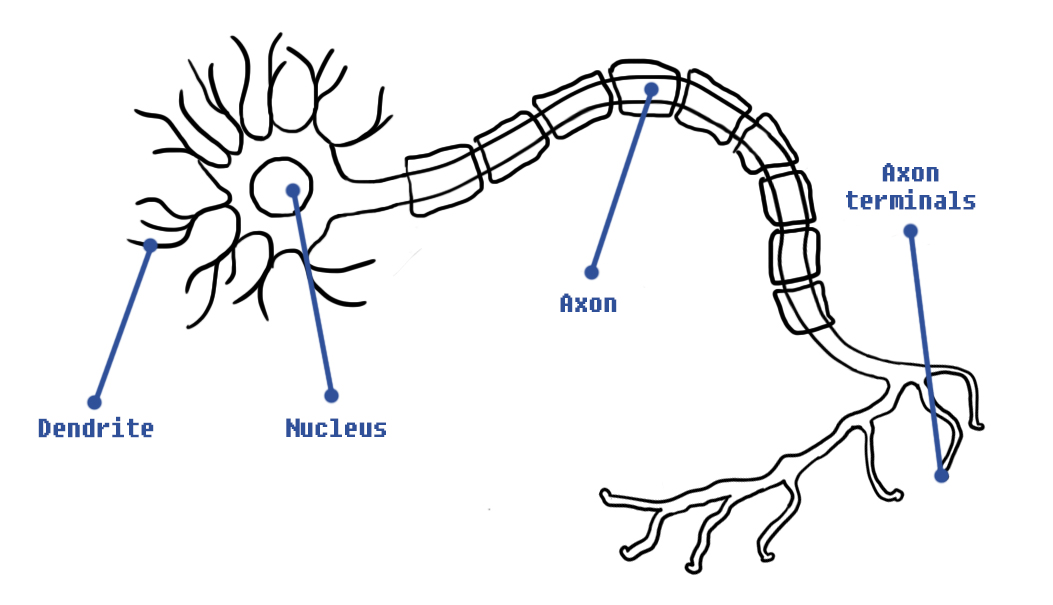
\includegraphics[width=10cm]{bio-neuron.jpg}
	\caption{Organic Neuron}
	\label{fig:org_neuron}
\end{figure}

The model of a neural network is a very simple concept. First, like a real neural network, \glspl{ann} are based in singular units called neurons, nodes or simplyly units. As we can see in the \textit{Figure ~\ref{fig:org_neuron}}, these neurons are composed by dendrites, a nucleus, an axon and axon terminals. To create a network is as simple as connecting two of this neurons with an axon terminal (output) of the first neuron to a dendrite (input) of the second.

ORGANIC NEURON FIGURE

Now going back to our artificial neural networks, we can see how the model of one of its units is pretty similar (\textit{Figure ~\ref{fig:art_neuron}}). In first place, the unit receives inputs ($x_i$) from an external source or from other units. Each of these inputs have an associated weight ($w_i$), assigned depending of its relative importance to the other inputs. After the unit applies a function $f$ to the weighted sum of its inputs, and finally it gives an output.

ARTIFICIAL NETWORK FIGURE

\begin{figure}[ht]
	\centering
	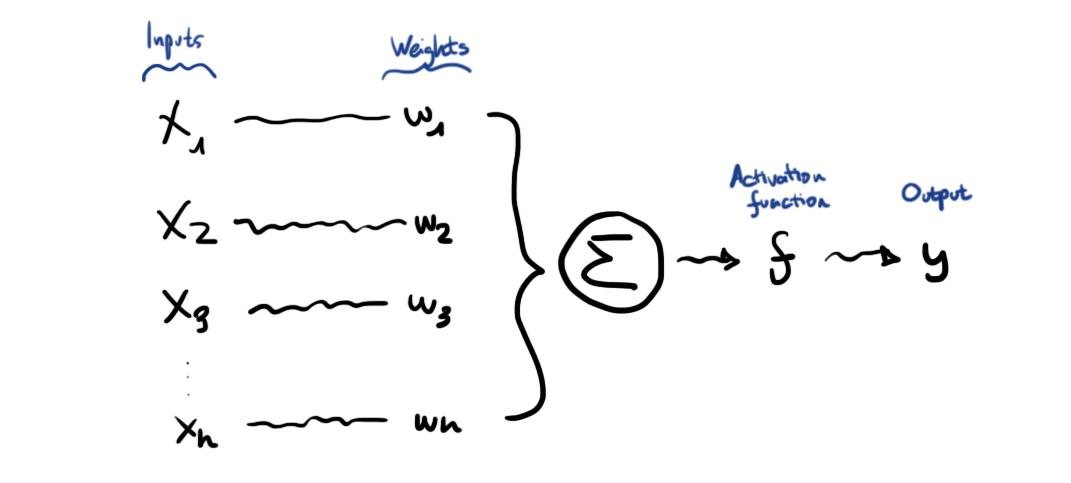
\includegraphics[width=\textwidth]{artificial-neuron.jpg}
	\caption{Artificial Neuron model}
	\label{fig:art_neuron}
\end{figure}

To construct a network we could connect two of this units as we did before with the neurons, but this time we are going to go one step forward creating a feedforward network. This network is divided in layers, so nodes from the same layer are not connected and between adjacent layers each connection has associated a weight. 

%%%%%%%%%%%%% CHANGE IMAGE %%%%%%%%%%%%%
\begin{figure}[ht]
	\centering
	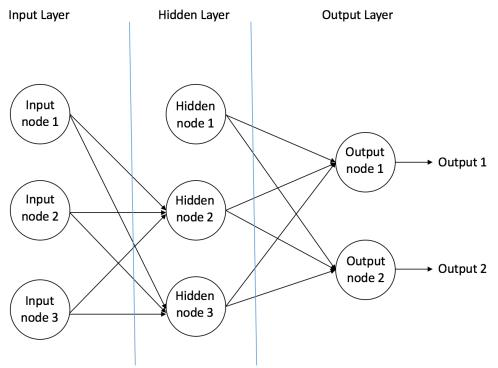
\includegraphics[width=\textwidth]{ann_basic_model.jpg}
	\caption{Basic Artificial Neural Network}
\end{figure}
%%%%%%%%%%%%%%%%%%%%%%%%%%%%%%%%%%%%%%%%

Because of the position of these nodes and the connections between them we can differentiate three types of nodes: input, hidden and output nodes.

\begin{itemize}
	\item Input Nodes: provide information from the outside world without computing anything, they just past the information to the hidden nodes. Collectively the nodes in this layer are referred to as the \textit{Input Layer}. 
	\item Hidden Nodes: they have no connection with the outside world (hence the name "hidden"), but they compute the information provided from the previous layer and give the output to the next one. Collectively the nodes in this layer are referred to as the \textit{Hidden Layer}. Although articial neural networks must have only one input layer and one output layer, they can have more than one hidden layer (or none). 
	\item Output Nodes: collectively the nodes in this layer are referred to as the \textit{Output Layer} and they are responsible to transfer the computed information to the outside world again.
\end{itemize}


\section{The perceptron}
Within the Artificial Neural Networks (\gls{ann}), we can find great variety of units that define the type of \gls{ann} involved, but in order to explain how they work, we are going to use a perceptron (shown in Figure 2.2). This unit has several inputs that are used to perform an operation involving all of them, to finally calculate a single value as a result in a single output.

Each input is composed of a value and a weight, which will contribute to the output of the perceptron. The operation involving all inputs is a linear combination:

\begin{equation}
    \label{linear_combination}
        f(x)=\sum_{i=0}^{n} w_n x_n = w_0 + w_1 x_1 + w_2 x_2 + w_3 x_3 + ...%
\end{equation}

where $x_n$ are the inputs of the perceptron and $w_n$ are the weights ($x_0=1$ is not an input, it's an useful constant to allow us to write the linear operation with a summatory). Finally, the (unique) output of the perceptron depends on the result of the linear operation, being 1 if the result is positive; or -1 in another case. All these data allow us to define the perceptron as follows:

\begin{equation}
    \label{perceptron_rule}
	perceptron(f(x)) =
		\begin{cases}
	     	1 & \text{if $f(x)>0$} \\
	        -1 & \text{otherwise} \\
		\end{cases}
\end{equation}

	\subsection{Linearly Separable attribute}
	This atribute refers to the fact that an hyperplane can separate (or not) the different output values of the perceptron, dividing the space in two sides where there is only one kind of output (1 or -1). To explain it better, we are going to use a percetron with two inputs. With this inputs we can produce a Cartesian map (first input would be X axis; and second input, Y axis). Instead of using a point to represent the input, we use the output symbol (``"+``" or ``"-``"). If we can draw a line (our hyperplane in a 2-dimension space) that divides the map in two sides, so that on each side of the line we can only find one kind of symbol (all positives or all negatives), then we can say that the set of points we have used is linearly separable.  
	
	With a single perceptron there are sets of points that can't be linearly separable. That's why networks of perceptrons with more than one layer are created, whose first layer perceptron's outputs is not the final result, but performs the role as input to another perceptron in the next layer. This way, even the non-linear surfaces can be represented.

	\subsection{Training Rule}
	In order to train perceptrons, we begin assigning random values to the weights and then we apply the perceptron to each training example. If the perceptron misclassifies an example, the training rule will modify the weights according to:

	\begin{equation}
		\label{training_rule}
		w_{i}^{'} \leftarrow w_{i} + \eta (t - o) x_{i}
	\end{equation}

	where $\eta$ is the \textit{learning rate} (constant usually small that determines how much weights vary in each step), $t$ is the target value, $o$ is the actual output that we have obtained from the perceptron and $x_{i}$ is the input value.

	The weights will converge to a value that classify correctly within a finite number of iterations if (and only if) examples are linearly separable and the $\eta$ value used is sufficiently small.
	
	\subsection{Delta Rule and Gradient Descent}
	When the input set is not linearly separable, we need an alternative to the training rule: delta rule. Delta rule uses gradient descent to search for the hypothesis space (set of outputs) that best fit the training example. 

	To explain this we’re going to use a linear unit (not thresholded as the perceptron) which output is calculated by $o = \vec{w} \cdot \vec{x}$. To measure the training error we’re going to use the next formula, where $D$ is the set of examples. It depends only of $\vec{w}$ because we assume that its relation with the examples set $\vec{x}$ will be gone after the training.

	\begin{equation}
		\label{error_function_full_square}
		E(\vec{w}) = \frac{1}{2} \sum_{d \varepsilon D} (t_d-o_d)^2 
	\end{equation}

	If error is defined by this formula, its representation (assuming two inputs) would be a parabolic surface with only one local minimum (as shown in fgure blabla). The gradient descent will start using a random initial vector and the algorithm will modify its direction step by step. In each step, the algorithm will choose the variation that go the deepest along the error surface. By this way, the process will continue until the local (and global minimum in this case) is reached.

	\begin{figure}[ht]
		\centering
		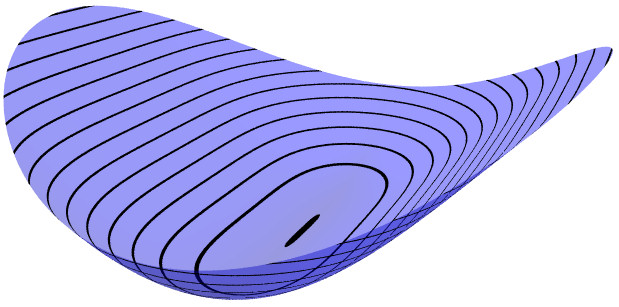
\includegraphics[width=\textwidth-30mm]{parabolic_surface.jpg}
		\caption{Parabolic Surface with one local minimum}
		\label{fig:parabolic_surf}
	\end{figure}

	\subsection{Derivation of Gradient Descent}
	To modify the direction of the vector we will derivate the error function ($E(\vec{w})$) respect of $\vec{w}$, form that is called \textit{gradient of E}:

	\begin{equation}
		\label{gradient_of_E}
		\nabla E(\vec{w})= [\frac{\partial{E}}{\partial{w_{0}}}, \frac{\partial{E}}{\partial{w_{1}}}, ..., \frac{\partial{E}}{\partial{w_{n}}}]
	\end{equation}

	This vector specifies the direction that produces the steepest increase in E, so including a negative factor ($-1$) we can calculate the steepest decrease in E. We can represent the training rule with its component form:

	\begin{equation}
		\label{training_rule_component_form}
		w_{i}^{'} \leftarrow w_{i} + \Delta w_{i} \hspace{1.5cm} ; \hspace{1.5cm} \Delta{w_{i}}=-\eta \frac{\partial{E}}{\partial{w_i}}
	\end{equation}

	So the final expression of the gradient descent is:

	\begin{equation}
		\label{gradient_descent_final_expr}
		\Delta w_i = -\eta \frac{\partial{E}}{\partial{w_i}} = \eta \sum_{d \varepsilon D} (t_d - o_d) x_{id}
	\end{equation}


	\subsection{Gradient Descent Algorithm}
	A brief version of the algorithm would be as follows:

	\begin{enumerate}

		\item Pick an initial random weight vector.
		\item Apply the linear unit to all training examples and then compute $\Delta w_i$  using the gradient descent formula.
		\item Update each weight adding $\Delta w_i$.
		\item If the algorithm hasn’t reached the local minimum, repeat from step 2.
	
	\end{enumerate}

	\subsection{Stochastic Approximation}
	Instead of using all the examples to update the weight each step (which could imply a lot of work) there is another option: incremental/stochastic gradient descent. This way we will approximate the gradient descent updating the weights with each training example:

	\begin{equation}
		\label{delta_rule}
		\Delta w_{i}= \eta (t - o) x_{i}
	\end{equation}

	So the error function must be changed to:

	\begin{equation}
		\label{error_function_stoc_square}
		E(\vec{w}) = \frac{1}{2} (t_d-o_d)^2 
	\end{equation}

\section{Multilayer Perceptron Networks}
A single perceptron can only express linear decision surfaces, so it is very limited for real life situations. In contrast, a multilayer network learned by the backpropagation algorithm can express a rich variety of non-linear decision surfaces, which are more suitable for that kind of problems.

	\subsection{Is a perceptron valid for MLP? The Sigmoid Unit}
	A perceptron unit is perfectly valid for a MLP, but its discontinuous threshold output make it not suitable at all for gradient descent. Also, as a linear unit, multiple layers of cascaded units will only produce linear functions. Then, another option is required: a \textbf{sigmoid threshold unit}. This unit works pretty similar to the perceptron, but has another function at the output to perform the threshold, which is called logistic or sigmoid function ($\sigma(y)$).

		\begin{equation}
			\label{sigmoid_function}
			\sigma(y) = \frac{1}{1+e^{-y}}
		\end{equation}

	This function increases monotonically and continuously with its input and is able to map a large input domain to a small range (0, 1) of outputs, reason because is usually called \textit{squashing function}. Finally, being easy derivable make it a really good choice for our task. 


	\subsection{Backpropagation Algorithm}
	The Backpropagation Algorithm learns the weights for a multilayer  network, given a network with a fixed set of units and interconnections. It uses gradient descent to minimize the squared error between the output and its target values of the network:

		\begin{equation}
			\label{squared_error_function_network}
			E(\vec{w}) = \frac{1}{2} \sum_{d \varepsilon D} \sum_{k \varepsilon outputs} (t_{kd}-o_{kd})^2 
		\end{equation}

	As we have changed the error function definition, the error surface will have more than one local minima (not as before with a single perceptron). This means that gradient descent may fail in order to find the global minima and only reach a local minima instead. Anyway, it has been proved to produce excellent results even with this problem.

	The stochastic version of the Backpropagation Algorithm, applied for each training example, would be:

		\begin{enumerate}

			\item Input the values in the network and obtain the output values computing every unit of the network.
			\item For each output unit ($k$), calculate its error term $\delta_k$, which is the usual $(t-o)$ multipied to the derivate of the sigmoid function:
				\begin{equation}
					\label{backpropagation_output_error}
					\delta_k \leftarrow o_k (1 - o_k)(t_k - o_k)
				\end{equation}				

			\item For each hidden unit ($h$), calculate its error term $\delta_h$. This is similar to the output formula, but as we don't have a target value for a hidden unit, we must calculate it summing up the errors of the downstream units weigthing each error by the weight of the connection that links them. 
				\begin{equation}
					\label{backpropagation_hidden_error}
					\delta_h \leftarrow o_h (1 - o_h) \sum_{l \varepsilon downstream} (w_{hl} \delta_i)
				\end{equation}

			\item Update each network weight:
				\begin{equation}
					\label{backpropagation_weight_update}
					w^{'}_{ji} \leftarrow w_{ji} + \Delta w_{ji} \hspace{1.5cm} ; \hspace{1.5cm} \Delta w_{ji} = \eta \delta_j x_{ji}
				\end{equation}

		\end{enumerate} 


\section{Convolutional Neural Networks and Face Recognition}
The Artificial Neural Networks (\glspl{ann}) we have seen until now have their applications, but the current state of the art for detecting what an image is (or what does it contains) are Convolutional Neural Networks (\glspl{cnn}). First of all we need to explain that this two kinds of neural networks are not at the same level. The \glspl{ann} we have seen until now usually have a few hidden layers, but \glspl{cnn} need to have multiple of these hidden layers in order to achieve what is known as Deep Learning. 

It may seem normal that adding more hidden layers to a network will improve its learning potential, but the problem with deep networks is that it becomes harder to learn the weights as the network becomes "deeper". In \cite{huang2016deep}, they mentioned this problem as \textit{Diminishing Feature Reuse} or \textit{Loss in the Information Flow}, explaining that the features of the input instance (or those computed by previous layers) are "washed out" in the proccess of learning, which makes it hard for later layers to learn meaningful gradient directions. Since the weights in the network are randomly initialised, it can become pretty hard (even impossible) to achieve learning in a deep neural network using backpropagation. Here is where Deep Learning comes into play, providing algorithms and architectures that helps in the training of such deep neural networks. 

Convolutional Neural Networks are one of the options Deep Learning provides. As \cite{lecun2015deep} explain, they are designed to proccess data that comes in the form of multiple arrays, which suits perfectly to our needs to work with images. For example, a colour image could be decomposed in three two-dimensions arrays that contain the pixel intensities in the three colour channel of RGB. 

%%% maybe include something from lecun paper, first page %%%

In terms of architecture, \glspl{cnn} are structured as a series of stages. First few stages are composed by convolutional and pooling layers (\cite{lecun2015deep}). 

Pooling is simple, it is just a down-sampling. We start with an image of a certain size, 30x30 pixels (which are just values from 0 to 255) for example. From this full image, taking it as a matrix, we select a window of a certain size. Usually we choose a size that makes possible to divide the full image in little windows that do not collide with each other. In this case, from a image of 30x30 we are going to take a 3x3 window, leaving us a total of 100 windows. 

Now, in each window we are going to perform a "max-pooling", which is to take the highest value of the window and output it to a new "image" in the position where the window was in the previous image. After doing this to all windows, we obtain a new image or matrix of 10x10, smaller than the initial one, but also with a worse quality.

%%%%%% INCLUDE IMAGE EXPAINING POOLING %%%%%%
image explaining pooling

Convolutional layers, in the other hand, follow a proccess more complex. They apply convolution (hence the name of the network) to the input image, which can be defined in a simple way as mixing information from two sources according to a specific rule. From the mathematical point of view, convolution is the integral of the element-wise multiplication of the two input functions. While it is complex itself, it is usually used to simplify even more complex equations. In our case we are going to work only with integers, so the convolution used here is a \textit{discrete convolution}. 

\begin{equation}
	\label{discrete_conv}
	f*g(n) = \sum_{m= -\infty}^{\infty} f(m) g(n-m) 
\end{equation}

If we apply this to the algorithm of a \gls{cnn}, the first input function would be a part of the image itself, that is called \textit{receptive field} or \textit{window}; and the second would be the \textit{filter}, which is a matrix of weights of the same size of the window. The result of this convolution is a \textit{feature map}, a new image that shows how the feature recognised by the filter is distributed in the original picture. 

If the image is in color, it is composed by the three different channels of the RBG standard, so the multiplication has to be applied to all of them. This element-wise multiplication in matrices has the name of Hadamard Product and it produces a matrix of the same size of the inputs. Once the multiplication is done, we have three matrices that we sum in one value. Now a function $f$ is applied to this output to finally obtain the value of the first pixel of the feature map. After that, the window moves one pixel to the right (or to the first pixel of the next row, if the end is reached) and applies again convolution to obtain the next pixel of the feature map. 

\begin{figure}[ht]
	\centering
	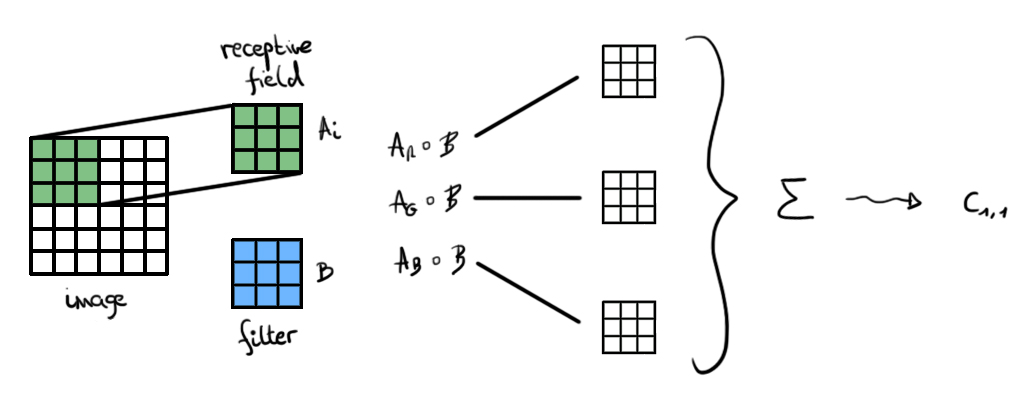
\includegraphics[width=\textwidth]{convolution.jpg}
	\caption{Convolution proccess for the creation of a Feature Map}
	\label{fig:convol_creation_feature_map}
\end{figure}

In the previous paragraph we said that a function $f$ is applied to the sum, as is usual in the structure of a neuron. Before \cite{krizhevsky2012deep}, the standard way to model this function was $f(x)=tanh(x)$. However, in this paper it is explained that these kind of saturating nonlinearities are much slower than a non-saturating nonlinearity as $f(x)=max(0, x)$. The neurons with this nonlinearity are called Rectified Linear Units or ReLUs, and help to train a deep convolutional network several times faster than their equivalents with $f(x)=tanh(x)$.

At this point, we know how convolution and pooling works. Two or three stages of convolution, followed by the non-linearity function, and then pooling; are stacked. After that, in the structure of a \gls{cnn} we find fully-connected layers, like a usual neural network, and finally an output layer that shows the prediction as the class with highest percenteage.

Backpropagation through a \gls{cnn} is as simple as through a regular deep network, allowing all the weights of the network (which also includes the filters of the convolution) to be trained.

\section{Face Detection}
The databases used in the training of the networks that perform the face recognition usually have face images already normalized  to  a  given  pose  standard. However,  the  conventional  input  image  of  computer  vision  systems  may  contain many items and/or faces, either for recognition or tracking. In these cases, face detection becomes mandatory. It acts as preprocessing of the images to determine first
if there is a face in the image, and second, where it is located (\cite{marques2010face}).

	\subsection{Limitations}
	Despite of the importance of the task, there are some limitations that strongly difficult it. First, any analysis that we perform on an image may be altered by the image’s resolution or noise. Such restricting factors can be mitigated by, for example, using a better quality equipment. However, other limitations to these techniques are even harder to overcome (\cite{yang2002detecting}):

	\begin{itemize}
		\item Pose. Face images may vary due to the relative position of the camera with respect to the face, resulting in a front, profile or even an inverted photo of the face.  
		\item Structural components. The presence or not of facial features such as moustaches and beards or accesories such as glasses may lead to not detect a face in the photo. Apart from the presence of the elements themselves, their wide diversity of shape, size and color also represent a limitation.  
		\item Facial expression. Certain facial expressions may distort a face so much that it cannot be detected.    
		\item Occlusion. The faces in the image may be partially covered by other objects or even other faces.
		\item Image orientation. Not only the portrait and landscape orientations, but also all the posible rotations that the image could have from what is expected in first place.
		\item Imaging conditions. In this section are included all factors that come from the construction of the photo, such as the illumination, for example.  
	\end{itemize}

	\subsection{Techniques}
	In order to perform the face detection in a photo, there are many different techniques among which to choose. In 1998, Henry A. Rowley and his team presented an approach based in the use of neural networks. In the Figure \ref{fig:rowley_network} we can see the algorithm followed to perfom the face detection on an image. Examining preprocessed small windows of a grayscaled image, a retinally connected network decides whether the window contains a face or not. The system arbitrates between multiple of these networks to improve the performance (\cite{rowley1998neural}). 

	\begin{figure}[h!b]
		\centering
		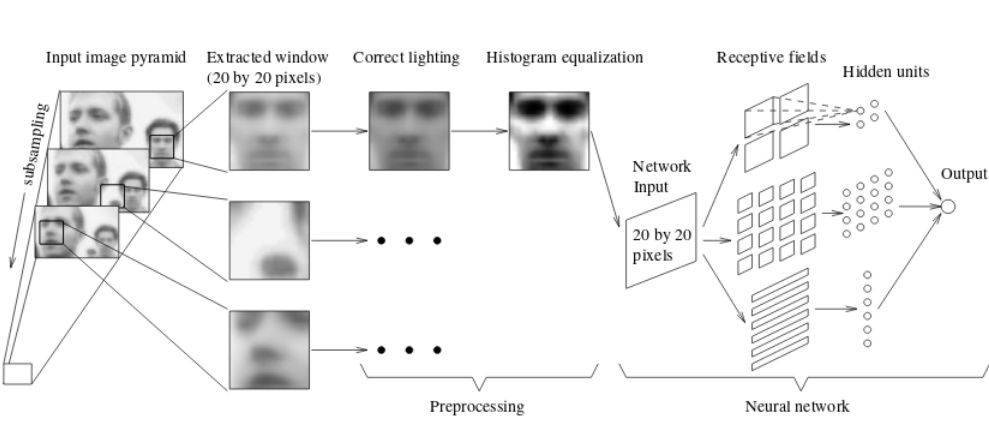
\includegraphics[width=13cm]{rowley_network.png}
		\caption{Basic algorithm used for face detection in \cite{rowley1998neural}}
		\label{fig:rowley_network}
	\end{figure}

	Another technique is presented in 2000 by Henry Schneiderman and Takeo Kanade for object detection, now using a statistical method (\cite{schneiderman2000statistical}). The inputs used here are still images, so to create visual attributes that are localized in space, frequency, and orientation, they needed to easily select information that is localized along these dimensions. The answer to this question was to perform a wavelet transform of the image. 

	Using a product of histograms, they represent the statistics of both object and "non-object" appearance. Each histogram represents the joint statistics of a subset of wavelet coefficients and their position on the object. Their approach was based in using many of these histograms in order to represent a wide variety of visual attributes. In the Figure \ref{fig:statistical_method_face_det} we can see how this method, in addition to detect the faces in the image, it also detects the direction to where the person is looking to.

	\begin{figure}[h!b]
		\centering
		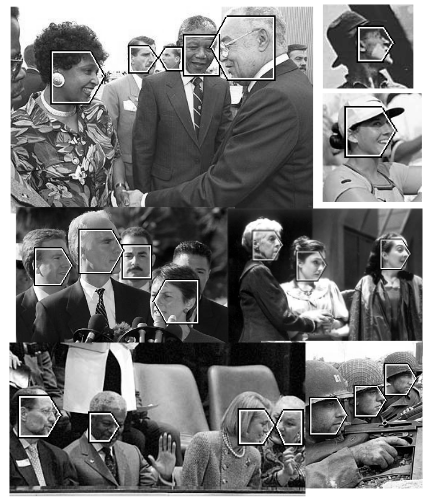
\includegraphics[width=8cm]{fd_statistical_method.png}
		\caption{Results of applying the face detection method from \cite{schneiderman2000statistical}}
		\label{fig:statistical_method_face_det}
	\end{figure}

	Finally, in 2001, Paul Viola and Michael Jones presented a framework for fast object recognition (\cite{viola2001rapid}). Althought it could be trained to detect a wide variety of objects, the main objective always was the face detection. It stands out for performing a high detection rate with a very low false positive rate and capable to work in a real time situation, such as face detection in video.

	This method has a total of 4 stages:
	
	\begin{enumerate}
		\item Obtaining Haar features. In the Figure \ref{fig:haar_features} we can see the Haar filters that are used to extract face features (Haar features in short) in the OpenCV library. Haar features work with the similarities that all human faces share and that are shown in a photo as a difference in the intensities of the pixels. For example, in the Figure \ref{fig:application_haar_features} an horizontal line Haar feature is applied for detecting the position of the eyes, as the pixels that represent them are way darker than the pixels that represent the cheeks. The same happen with the vertical line Haar feature in the same figure, dectecting the dark pixels of the eyebrows and the brighter ones for the space in the middle. The use of Haar filters was motivated by the work of \cite{haar_features_before_vj}, but in this case they do not work directly with image intensities. 

		\begin{figure}[h!b]
			\centering
			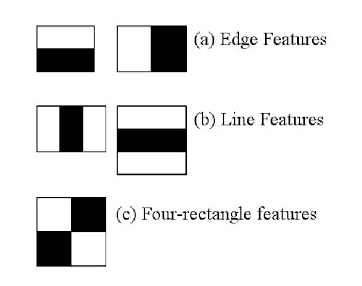
\includegraphics[width=8cm]{types_haar_features.png}
			\caption{Different types of Haar features (\cite{opencv_haar_cascade_tut})}
			\label{fig:haar_features}
		\end{figure}

		\begin{figure}[h!b]
			\centering
			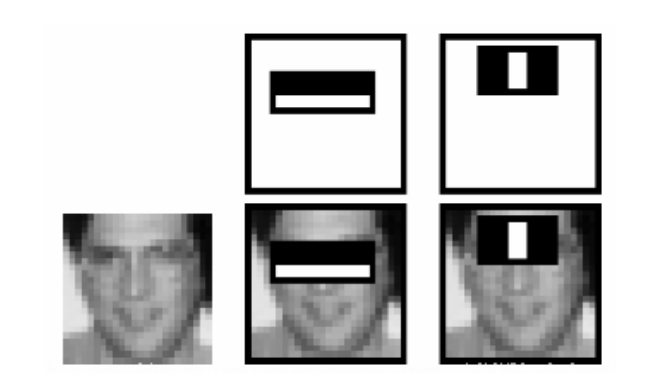
\includegraphics[width=8cm]{application_haar_features.png}
			\caption{Application of Haar features to an image (\cite{viola2001rapid})}
			\label{fig:application_haar_features}
		\end{figure}

		\item Analysis of the Haar features. The Haar features are computed very rapidly using an intermediate representation for the image called \textit{integral image} (also known as Summed Area Table (\cite{crow_summed_table})), obtaining the sum of all the values in the rectangular area of the feature. 

		\item Training with AdaBoost. A variant of the AdaBoost learning algorithm is used to select a small set of features, as the cost of using all features would be too high, and to train the classifier. A \textit{strong} classifier is built as a lineal combination of weak classifiers, which are focused in a single rectangle feature each. The objective of the training is to adjust the weights used in order to minimise false negatives. A \textit{weak} classifier $h_j(x)$ thus consist of a feature $f_j$, a threshold $\theta_j$ and a parity $p_j$ indicating the direction of the inequality sign:

		\begin{equation}
			\label{eq:viola_jones_weak_classifier}
			h_j(x)=
				\begin{cases}
			     	1 & \text{if $p_jf_j(x) < p_j\theta_j$} \\
			        0 & \text{otherwise} \\
				\end{cases}
		\end{equation}

		\item Cascade architecture. The main idea of this stage is to build a degenerated decission tree (called \textit{"cascade"} in the article) using strong classifiers like the one we can see in the Figure \ref{fig:cascade_decission_tree}. Image sub-windows are feeded to this cascade, so if a face is detected by the first classifier, it triggers the evaluation of the second classifier. A positive result in the sencond triggers a third classifier, and so on. If a face is not detected in one of the classifiers, the sub-window is rejected. 
		
		\begin{figure}[h!b]
			\centering
			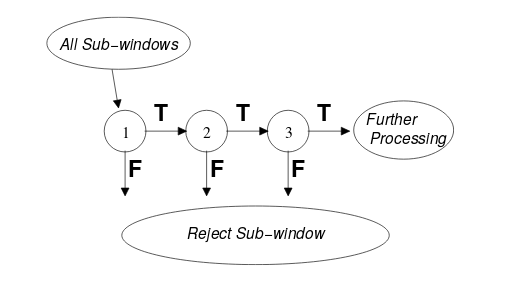
\includegraphics[width=10cm]{cascade_decission_tree.png}
			\caption{Schematic depiction of a the detection cascade (\cite{viola2001rapid})}
			\label{fig:cascade_decission_tree}
		\end{figure}
			
	\end{enumerate}

\section{Public Data Sets} 
Face recognition is nothing but another kind of machine learning and as such, it needs to be feeded with data, face images in this case. The problem is that we need a high amount of them, in addition to that each face image has to be different (or the model would only work well with the data we worked with, and not any face, which is our purpose). As we cannot generate this dataset by ourselves, we must look for a public dataset with enough and different face images:

\begin{itemize}
	\item CASIA Webface Database. It is the second largest database of faces (first is private and belongs to Facebook), with more than 10,000 subjects and almost 500,000 images. In order to use it an agreement needs to be signed so the database will only be used for non-comercial, research or educational purposes. We finally discarded it because its size, which would be more suitable for a big project with a research group (\cite{casia_db}). 
	\item WIDER FACE. This database counts with more than 32,000 images and can be freely accessed by a Google or Baidu Drive. It has the advantage that its images are already labelled and the faces in them are marked. However, many of the images have more than one face on them (they say they count with almost 400,000 faces in the dataset) and we need them to have only one person (\cite{widerf_db}).
	\item Labelled Faces in the Wild (LFW). This database only counts with more than 13,000 images that only have one person in them, which is perfect for the scope of this project. It can be explored online and has been recently updated, solving some erratum. Finally, it also has the option to download the images aligned with funneling or commercial software, reducing the work to do on the dataset. Because of all these reasons, it is the dataset that is going to be used for the project (\cite{lfw_db}).
\end{itemize}

\section{Raspberry Pi}	
The Raspberry Pi was designed by scientists from the University of Cambridge and realeased their first commercial model in 2012. At the first instance it was thought to be a programming learning tool accessible for everyone thanks to the low cost of the device (\cite{raspberry_pi_for_learning}), now around the 40e (\cite{price_raspberry_pi}). However, a huge community has grown around this project that goes from the original purpose of programming learning to industrial and comercial products.

	\subsection{Specifications}
	All the specifications of this device can be found in the table \ref{table:rasp_pi_specs}. For this project a camera will be needed to take photos of the users. There are a lot of camera models available for the Raspberry Pi with no big differences of performance in the scope of this \gls{fyp}. However, the Camera Module V2 (8 Megapixels) was finally chosen above the rest because it is the official camera for the Raspberry and has been used in many other projects. It counts with a Sony Exmor IMX219 Sensor and it is capable to record up to 1080p at 30fps.

	\renewcommand{\arraystretch}{1.3}
	\begin{table}[h!b]
		\centering
	    \begin{tabular}{| l | l |}
	    \hline
	    Model name & Raspberry Pi 3 Model B \\\hline
	    \multirow{2}{*}{Processor} & Chipset Broadcom BCM2387 \\ \cline{2-2}
                             	   & CPU Quad-Core 1,2GHz ARM Cortex-A53 \\\hline
		GPU & Dual Core Broadcom VideoCore IV \\\hline
		RAM memory & 1GB LPDDR2 \\\hline	    	    			
		\multirow{7}{*}{Connectivity} & Ethernet socket 10/100Mbps BaseT \\ \cline{2-2}
                             	   & \makecell[tl]{BCM43438 chip, providing 802.11 b/g/n wireless \\ LAN and Bluetooth 4.1 (Classic and BLE)} \\ \cline{2-2}
                             	   & 4x USB ports 2.0 \\ \cline{2-2}
                             	   & 40-pin extended GPIO \\ \cline{2-2}
                             	   & \makecell[tl]{CSI-2 camera port for connecting a Raspberry \\ Pi camera (15 pins)} \\ \cline{2-2}
                             	   & \makecell[tl]{DSI display port for connecting a Raspberry \\ Pi touchscreen display (15 pins)} \\ \cline{2-2}
                             	   & \makecell[tl]{Micro-SD port for OS and storage (power \\ source up to 2.5A)} \\\hline
        \multirow{2}{*}{Video output} & Full size HDMI (rev 1.3 \& 1.4) \\ \cline{2-2}
                             	   & Composite RCA (PAL \& NTSC) \\\hline
        Audio output & 3.5mm jack conector \\\hline
	    \end{tabular}
	    \caption{Specifications of the Raspberry Pi 3 Model B}
	    \label{table:rasp_pi_specs}
	\end{table}
	\renewcommand{\arraystretch}{1}

%	\begin{itemize}
%		\item Model name: Raspberry Pi 3 Model B
%		\item Processor:
%			\begin{itemize}
%				\item Chipset Broadcom BCM2387.
%				\item CPU Quad-Core 1,2GHz ARM Cortex-A53.
%			\end{itemize}
%		\item GPU: Dual Core Broadcom VideoCore IV.
%		\item RAM memory: 1GB LPDDR2.
%		\item Conectivity:
%			\begin{itemize}
%				\item Ethernet socket 10/100Mbps BaseT.
%				\item BCM43438 chip, providing 802.11 b/g/n wireless LAN and Bluetooth 4.1 (Classic and BLE).
%				\item 4x USB ports 2.0.
%				\item 40-pin extended GPIO.
%				\item CSI-2 camera port for connecting a Raspberry Pi camera (15 pins).
%				\item DSI display port for connecting a Raspberry Pi touchscreen display (15 pins).
%				\item Micro-SD port for OS and storage (power source up to 2.5A).
%			\end{itemize}
%		\item Video output:
%			\begin{itemize}
%				\item Full size HDMI (rev 1.3 \& 1.4).
%				\item Composite RCA (PAL \& NTSC).
%			\end{itemize}
%		\item Audio output: 3.5mm jack conector.
%	\end{itemize}

	\subsection{Possible Operative System}
	In order to use the Raspberry Pi in this project, we first need to install an Operative System (OS). There are many possible options and, not a surprise, most of them are Linux-based:

	\begin{itemize}
		\item Raspbian. The official OS for Raspberry Pi based on the popular Debian distribution of Linux. Apart from the usual tools every OS provide to make the Raspberry run, Raspbian include more than 35.000 packages specifically optimised for this small machine (\cite{raspbian_main_website}). It has become the most popular OS for a general purpose project in the Raspberry. 
		\item Ubuntu Mate. Canonical, the maker of Ubuntu, released this version for the Raspberry Pi swapping out the Unity desktop interface for a lighter version called "Mate". It is bigger than Raspbian and will require a microSD card of 6GB or greater, which is recommended to be a Class 6 or Class 10 in order to avoid a bottleneck (\cite{ubuntu_mate_review}).
		\item ArchLinux ARM. It is the port of the desktop version of ArchLinux to the ARM architecture. The basic installation of this OS only comes with the Linux kernel, a shell and the package manager, so users must install all the packages they need manually (\cite{archlinux_arm_main_website}).
		\item Kali Linux. Another port from a desktop version OS to the ARM architecture, Kali Linux in this case. Like the desktop version, it is the distribution of choice for penetration testings and forensics analysis, as it comes with well-known tools for these purposes (\cite{kalilinux_website}).
		\item PiBang Linux. Insired by Crunchbang Linux, and based on Rasbian, it aims at being a fully functioning desktop. It features a modified version of Raspi-Config along with a fully optimized Openbox install (\cite{pibang_website}).
	\end{itemize} 

\section{Python}
\label{sec:python}
Some of the features of Python have been already commented in the Introduction of this report, but there is more to talk about. Some people say that in order to explain something well, you need to start from the root of the question. If we apply it to Python, we have to talk about the Zen of Python (\cite{origin_zen_of_python}, \cite{zen_of_python}), a collection of software principles that influenced the design of this language. A total of 20 principles (of which only 19 were written down) that show how Tim Peters, one of the open source development leaders of Python, wanted it to be beatiful, explicit, simple among other thigs.

The readability of Python was also in these principles and we can find many aspects of the language that confirm this feature. One that really impressed me at the first place was the lack of brackets ("\{\}"), which are the usual way to delimit control flow blocks in other languages. Instead of brackets, Python uses indentation. To indicate that a line is inside a function or an block (an \textit{if} block in the example), we just have to indent it one level deeper. We can see it clearly in the next comparative.

\noindent\begin{minipage}[t]{.45\textwidth}
\begin{lstlisting}[caption=C code,frame=tlrb, language=C]{Name}
void foo(int x)
{
    if (x == 0) {
        bar();
    } else {
        foo2(x + 3);
    }
}
\end{lstlisting}
\end{minipage}\hfill
\begin{minipage}[t]{.45\textwidth}
\begin{lstlisting}[caption=Python code,frame=tlrb, language=Python]{Name}
def foo(x):
    if x == 0:
        bar()
    else:
        foo2(x + 3)
\end{lstlisting}
\end{minipage}

Another feature of Python is that it is interactive, which means that we do not need to write a Python program in a file to execute it later althought is also an option. Alternatively, we can interact with the prompt directly by executing the Python shell in the terminal. Also related with it, Python is interpreted, so it does not have to be compiled before executing (what happens to languages like C, C++ or Lisp). It is processed at runtime by the interpreter (\cite{python_overview}). 

Finally, the most important feature of Python: it is very easy to learn. It has fewer keywords than other languages, its strucure is much simpler and the syntax is can be easily understood with a certain level of English. 

These reasons have brought Python to be very popular. When looking at different sites, the ranking of the most popular languages can vary depending on the parameters that have been used for the calculations. The TIOBE Programming Community index in the Figure \ref{fig:tiobe_rank} shows a rank based in the hits for the search query, using engines like Google, Yahoo, or Wikipedia (\cite{tiobe_index_def}). The PYPL PopularitY is another rank that we can find in the Figure \ref{fig:pypl_rank}, which was created by analyzing how often language tutorials are searched on Google. The last one but not less important is the rank from the Github Octoverse, in the Figure \ref{fig:github_octoverse_rank}, which shows the number of pull request during 2017.

\begin{figure}[h!b]
	\centering
	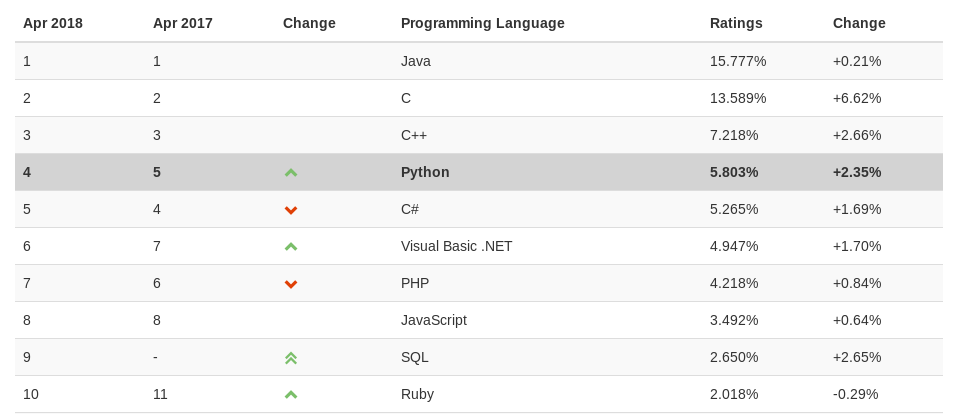
\includegraphics[width=13cm]{TIOBE_python_ranking.png}
	\caption{TIOBE Index for April 2018 (\cite{tiobe_index})}
	\label{fig:tiobe_rank}
\end{figure}

\begin{figure}[h!b]
	\centering
	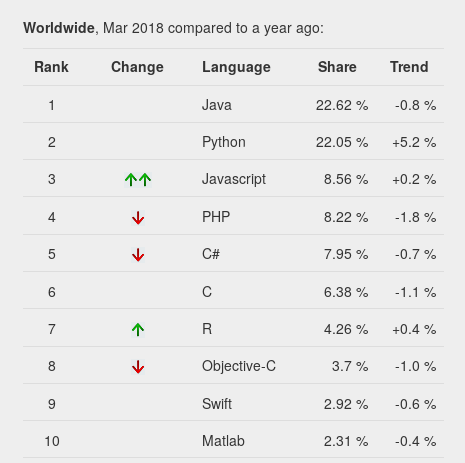
\includegraphics[width=9cm]{PYPL_python_ranking.png}
	\caption{PYPL PopularitY for March 2018 (\cite{pypl_pop_rank})}
	\label{fig:pypl_rank}
\end{figure}

\begin{figure}[h!b]
	\centering
	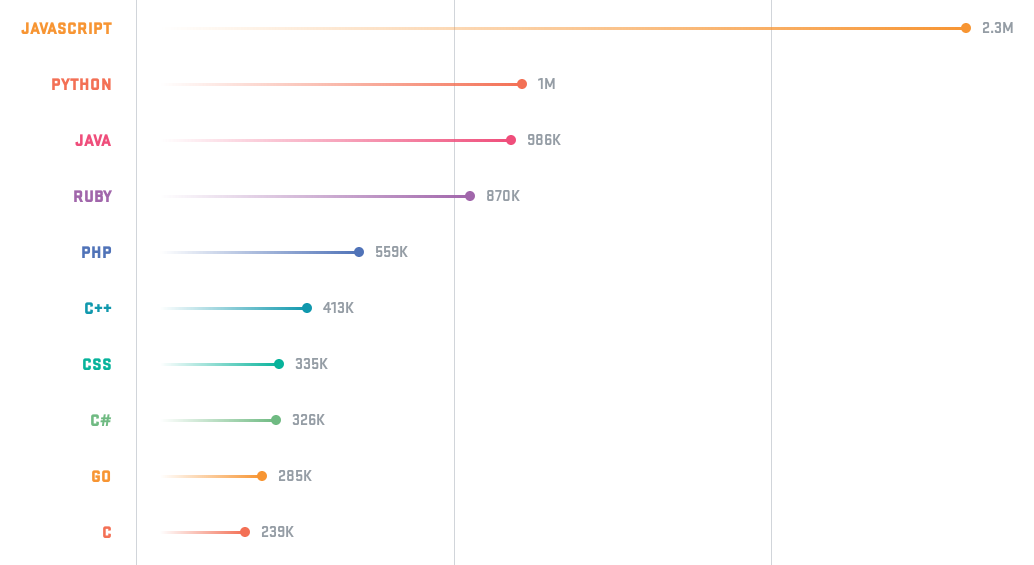
\includegraphics[width=13cm]{Github_python_ranking.png}
	\caption{Pull requests in Github for 2017 (\cite{octoverse_2017})}
	\label{fig:github_octoverse_rank}
\end{figure}

All rankings show the healthy condition in which Python is at the moment, being in the top 5 languages in all of them. second in two of them and fourth in the other one. It has even unseat Java as the second-most popular language in GitHub, with 40 percent more pull requests opened this year than last (\cite{octoverse_2017}). 